\documentclass[manuscript,screen]{acmart}

\setcopyright{none}
\settopmatter{printacmref=false}
\renewcommand\footnotetextcopyrightpermission[1]{}
\acmConference[Mid-Semester Review Paper]{Mid-Semester Evaluation}{September 2026}{Indian Institute of Information Technology}
\acmYear{2026}

\usepackage{amsmath}
\usepackage{booktabs}
\usepackage{tabularx}
\usepackage{array}
\usepackage{tikz}
\usetikzlibrary{arrows.meta,positioning,shapes.geometric,fit,calc}
\usepackage{enumitem}
\usepackage{multirow}

\newcolumntype{Y}{>{\raggedright\arraybackslash}X}

\title{Knowledge Cutoff Effects on LLM-Generated Literature Reviews in Rapidly Evolving Fields}

\author{Aman Tiwari}
\affiliation{%
  \institution{Indian Institute of Information Technology}
  \country{Prayagraj}
  \country{India}}

\begin{document}

\begin{abstract}
Large language models (LLMs) are increasingly used to support literature discovery, synthesis,
summarization, and the preparation of research reviews. Their usefulness, however, is constrained by a
fundamental temporal asymmetry: scientific knowledge evolves continuously, whereas a conventional
pretrained model acquires most of its parametric knowledge from a finite historical training corpus. This
temporal mismatch is particularly consequential in rapidly evolving fields such as artificial intelligence,
biomedicine, climate science, cybersecurity, and emerging technologies, where important findings,
terminology, datasets, methods, and consensus positions may change substantially within months. This
review examines how knowledge cutoffs affect LLM-generated literature reviews and argues that the problem
extends beyond simple omission of recent papers. Cutoffs can distort literature coverage, citation selection,
interpretation of research trends, assessment of methodological consensus, and identification of research
gaps. The review synthesizes research on temporal knowledge, retrieval-augmented generation (RAG),
continual learning, knowledge editing, hallucination, citation reliability, and automated scientific literature
synthesis. Current approaches—including scholarly retrieval, temporal filtering, continual updating, model
editing, agentic research systems, and citation verification—reduce some cutoff effects but do not eliminate
temporal misalignment. The central research gap is the lack of evaluation that treats time as a first-class
property of scholarly evidence. Future systems therefore require timestamp-aware retrieval, source
provenance, temporal reasoning, claim-level citation verification, uncertainty estimation, conflict resolution,
and reproducible search logs.
\end{abstract}

\keywords{large language models, knowledge cutoff, literature review, scientific literature synthesis, temporal knowledge, retrieval-augmented generation, citation reliability, continual learning, research agents, temporal alignment}

\ccsdesc[500]{Computing methodologies~Natural language processing}
\ccsdesc[500]{Information systems~Digital libraries and archives}
\maketitle

\section{Introduction}\label{sec:introduction}
Literature reviews organize existing evidence, identify methodological developments, expose disagreements,
and establish the rationale for new investigations. Traditionally, preparing a high-quality review requires
iterative database searching, screening, reading, comparison, citation management, and expert synthesis.
The growth of scientific publication has made this process increasingly difficult for individual researchers.
Recent work on automated literature research explicitly identifies publication volume as a major bottleneck
and motivates LLM-based review-generation systems as a way of reducing the associated cognitive burden
\cite{wu2025}.

LLMs have changed this workflow by allowing researchers to ask questions in natural language and receive
summaries, comparisons, explanations, and draft reviews. However, conventional LLMs are not continuously
synchronized with the scholarly record. Their parametric knowledge is primarily acquired during pretraining,
and a model with a training cutoff cannot inherently know papers, discoveries, terminology, or empirical
results that emerged afterward. Retrieval-augmented generation (RAG) addresses part of this limitation by
combining parametric model knowledge with an external non-parametric memory that can be updated
independently of model weights \cite{lewis2020}.

The knowledge-cutoff problem is more complicated than asking whether an LLM ``knows'' a recent paper.
Cheng et al. show that the effective cutoff of an LLM can differ from its nominally reported cutoff because
training corpora contain documents with different temporal properties \cite{cheng2024}. Older material can
remain present in later web crawls, while deduplication and corpus construction can create additional temporal
inconsistencies. Thus, model knowledge is better understood as a temporal distribution than as a single date.

For literature reviews, this distinction is particularly important. A review is not merely a collection of
facts; it is a structured representation of how a field has developed. If an LLM misses recent studies, it can
misrepresent the current state of evidence, incorrectly identify an old problem as unsolved, fail to recognize a
newly established method, overstate the importance of obsolete techniques, or describe a historical research
debate as if it were current. Knowledge-cutoff effects can therefore become epistemic distortions rather than
ordinary factual errors.

This paper addresses five questions:
\begin{enumerate}[leftmargin=*]
    \item How do knowledge cutoffs influence LLM-generated literature reviews?
    \item Why are rapidly evolving fields especially vulnerable?
    \item Which technical approaches mitigate temporal limitations?
    \item What new failure modes arise when retrieval and agentic systems are introduced?
    \item What evaluation and architectural principles are required for temporally reliable review systems?
\end{enumerate}

The paper is a conceptual and narrative synthesis of scholarly research available through August 2026. It
does not claim to be a systematic review of every publication on LLM-assisted literature review. Instead,
it integrates research from temporal reasoning, RAG, continual learning, scientific literature synthesis,
hallucination, citation verification, and research-agent evaluation. Section~\ref{sec:background} establishes
the conceptual foundations, Section~\ref{sec:distortions} analyzes the distortions caused by temporal
misalignment, and Section~\ref{sec:approaches} compares mitigation approaches.

\section{Background and Related Work}\label{sec:background}

\subsection{Parametric knowledge and the knowledge cutoff}\label{subsec:parametric}
Modern LLMs store statistical representations of language and world knowledge in their parameters. This
design provides broad generalization capabilities but creates a separation between model knowledge and
current external knowledge. RAG formalizes a complementary relationship between parametric and
non-parametric memory \cite{lewis2020}.

A nominal knowledge cutoff is therefore best understood as an approximation to the latest point in time
represented by the training distribution. Cheng et al. demonstrate that the effective boundary can vary by
source and topic \cite{cheng2024}. A model may have detailed knowledge of an older research area while
having little representation of a newly emerging subfield. Conversely, some newer facts may occur in its
training distribution even when its nominal cutoff is earlier.

\subsection{Temporal knowledge and evolving facts}\label{subsec:temporal}
Temporal knowledge has become an active research problem. Kim et al. evaluate world knowledge in lifelong
language models and show difficulties associated with evolving information \cite{kim2024}. Zhang and Choi
frame the issue as temporal misalignment: a model trained on historical data may be asked questions about
the present. Their fact-duration approach estimates how long facts are likely to remain valid and uses that
information to reduce the impact of stale knowledge \cite{zhang2023}.

More recent benchmarks extend evaluation beyond static factual recall. EvolveBench evaluates temporal
competence through dimensions including temporal awareness, trustworthiness, understanding, and reasoning,
while HoH examines the effect of outdated information in retrieval-based settings \cite{zhu2025,ouyang2025}.
These results indicate that temporal reliability cannot be reduced to model size or general reasoning ability.
A model may reason well while still failing to determine whether a claim is valid at the requested point in time.

\subsection{Hallucination and citation reliability}\label{subsec:hallucination}
Knowledge cutoffs interact with hallucination. When a model cannot retrieve a recent paper, it may generate a
plausible but unsupported description of what the literature contains. More generally, LLM-generated text can
contain unsupported or factually inconsistent information \cite{ji2023,maynez2020}.

The problem is especially important for academic writing because literature reviews require citations. Walters
and Wilder evaluated ChatGPT-generated bibliographic citations and documented fabricated and erroneous
references \cite{walters2023}. Citation existence and citation validity should therefore be distinguished. A
citation may point to a real paper while failing to support the attached claim. Conversely, a genuine older paper
may be cited because a newer study is inaccessible, producing a formally valid but temporally incomplete review.

The cutoff problem can consequently be decomposed into three related dimensions:
\begin{itemize}[leftmargin=*]
    \item \textbf{Coverage error:} important recent literature is missing.
    \item \textbf{Temporal attribution error:} a valid source is presented as representing current knowledge when it represents an earlier state.
    \item \textbf{Citation error:} a reference is nonexistent, bibliographically inaccurate, or weakly entailed by the cited source.
\end{itemize}

\subsection{LLMs in literature-review workflows}\label{subsec:workflow}
LLM use in evidence synthesis increasingly extends beyond simple summarization. A scoping review identified
applications across 10 of 13 systematic-review stages, with literature search, study selection, and data
extraction among the most frequent uses, while fully validated applications remained uncommon
\cite{lieberum2025}.

Systems such as LitLLM use search, keyword generation, reranking, and RAG to construct related-work
sections \cite{agarwal2024}. PaperQA demonstrates retrieval across full-text scientific papers for
evidence-grounded question answering and synthesis \cite{lala2023}. These systems mark a transition from
closed-book generation toward evidence-grounded research assistance, but the evidence itself still requires
temporal and bibliographic validation.

\section{How Knowledge Cutoffs Distort Literature Reviews}\label{sec:distortions}

\subsection{Incomplete temporal coverage}\label{subsec:coverage}
The most direct consequence of a knowledge cutoff is missing literature. In a rapidly evolving field, papers
published after training may contain new benchmark results, limitations, methodologies, datasets, competing
approaches, replications, negative findings, or corrections to previously accepted conclusions. Omission is
therefore not temporally neutral: missing a recent study can change the direction of a review.

Fluent generation can conceal this incompleteness. A review may appear comprehensive because the prose is
coherent even though the evidence base is incomplete. This creates a particularly important scholarly risk:
stylistic quality can be mistaken for temporal coverage.

\subsection{Citation-lag bias}\label{subsec:citationlag}
Scientific influence is not synchronized with publication date. New papers often have few citations, whereas
older papers accumulate citations over time. Automated literature systems that use citation counts or citation
networks as proxies for importance may therefore favor established literature. Wu et al. explicitly identify
citation lag as a challenge for automated review generation in rapidly evolving fields \cite{wu2025}.

The resulting review can become ``popular-paper-centric'' rather than state-of-the-art-centric. Retrieval
probability may depend on age, citation count, indexing history, visibility, and textual prominence in addition
to topical relevance.

\subsection{Stale consensus}\label{subsec:stale}
A cutoff can preserve an older consensus. Suppose a field historically concluded that Method A was superior
to Method B, while later studies show that Method B performs better under realistic conditions. A cutoff-limited
LLM may continue to describe Method A as state of the art. This is not necessarily a hallucination: the model
may produce a historically accurate statement using genuine sources. The error lies in temporal framing.

The distinction can be expressed as a two-dimensional validity condition:
\begin{equation}
    \mathrm{Valid}(c,s,t)=\mathrm{Evidence}(c,s)\times\mathrm{TemporalFit}(s,t),
    \label{eq:temporal-validity}
\end{equation}
where $c$ is a claim, $s$ is its supporting source, and $t$ is the reference time. Equation~\eqref{eq:temporal-validity}
illustrates why factual correctness alone is insufficient for a current literature review.

\subsection{Distorted research gaps}\label{subsec:gapsdistorted}
Identifying research gaps is one of the most valuable functions of a review, but it is highly vulnerable to
cutoff effects. A system may state that few studies investigate a problem when several relevant studies were
published after its training cutoff. This creates false novelty and can encourage duplicated research. The
reverse can also occur: a model may identify a historical gap that recent work has already addressed.

\subsection{Misinterpretation of research trends}\label{subsec:trends}
A literature review should explain what methods dominated earlier research, what changed, why the change
occurred, which findings have been replicated, which approaches are emerging, and what remains uncertain.
A static LLM is poorly suited to these questions without explicit temporal evidence. Findings from temporal
benchmarks reinforce this limitation \cite{kim2024,zhu2025}.

\subsection{Changing terminology}\label{subsec:terminology}
Rapidly evolving fields frequently change terminology. A cutoff-limited model may fail to recognize a new
term, interpret it using an older definition, miss papers because retrieval queries use obsolete terminology,
or incorrectly merge historically distinct concepts. The problem is particularly consequential in
interdisciplinary areas where terminology evolves faster than indexing systems.

\subsection{Conflicting temporal evidence}\label{subsec:conflict}
Adding retrieval does not automatically solve the problem. A retrieval corpus may contain multiple versions of
the same information: a preprint, conference paper, journal article, correction, retraction, or later replication.
A system must determine not only which source is relevant, but which source is temporally and scientifically
authoritative.

HoH demonstrates that outdated information in a retrieval knowledge base can reduce accuracy even when
current information is also available \cite{ouyang2025}. RAG therefore changes the question from ``Does the
model know the latest information?'' to ``Can the system retrieve, rank, reconcile, and correctly attribute
information according to time?''

\section{Current Approaches and Developments}\label{sec:approaches}

\subsection{Retrieval-augmented generation}\label{subsec:rag}
RAG retrieves external documents and conditions generation on the retrieved evidence \cite{lewis2020}. A
simplified literature-review pipeline is represented by
\begin{equation}
    Q \xrightarrow{R(\cdot,D)} C \xrightarrow{G(\cdot,Q)} A,
    \label{eq:rag-pipeline}
\end{equation}
where $Q$ is the research question, $D$ is the external corpus, $R$ is retrieval, $C$ is retrieved context,
and $G$ is generation producing answer or review $A$. RAG allows the underlying model to remain unchanged
while the evidence corpus is updated, but retrieval quality becomes a critical dependency.

\subsection{Scholarly RAG}\label{subsec:scholarly-rag}
General web search is not necessarily sufficient for scholarly review generation. Scientific systems need
metadata, abstracts, full text, publication dates, versions, citations, author information, and persistent
identifiers. PaperQA is an early research-oriented example \cite{lala2023}. OpenScholar is a more recent
specialized system backed by a large scientific datastore and combines retrieval, reranking, and iterative
self-feedback \cite{asai2026}. Its results illustrate that evidence infrastructure and architecture can be as
important as model scale for scientific synthesis.

\subsection{Temporal filtering and time-aware retrieval}\label{subsec:filtering}
Temporal filtering makes the reference time explicit. For a review describing the state of a field as of 2023,
post-2023 evidence should not be used as if it were available at that time. Conversely, a current review should
prioritize recent evidence. A time-aware retrieval score can be written as
\begin{equation}
    S(d)=\alpha R(d,q)+\beta T(d,t)+\gamma A(d)+\delta C(d),
    \label{eq:temporal-score}
\end{equation}
where $R$ is semantic relevance, $T$ is temporal relevance to reference time $t$, $A$ is source authority,
and $C$ is scholarly significance. Equation~\eqref{eq:temporal-score} formalizes the idea that a highly cited
but obsolete paper should not automatically outrank a recent and directly relevant study.

\subsection{Continual learning}\label{subsec:continual}
Continual-learning research distinguishes continual pretraining, domain-adaptive pretraining, and continual
fine-tuning \cite{wu2024,shi2024}. The advantage is that new knowledge becomes part of the model's internal
representation. Disadvantages include computational cost, catastrophic forgetting, and changing model behavior.
For literature-review systems, continual updating also introduces reproducibility problems: two researchers
querying the ``same'' system at different times may obtain different reviews.

\subsection{Knowledge editing}\label{subsec:editing}
Knowledge editing modifies selected model representations rather than retraining the entire model. Yin et al.
argue that outdated knowledge should not simply be erased because historical information remains useful for
historical questions \cite{yin2024}. Their temporal knowledge-editing formulation emphasizes preserving
historical knowledge while integrating new knowledge. This distinction is important for reviews, which should
explain the development of a field rather than overwrite its history.

\subsection{Fact-duration modeling}\label{subsec:duration}
Zhang and Choi propose predicting how long facts remain valid and using volatility to determine when external
information should be sought \cite{zhang2023}. The principle can be extended from facts to scholarly claims:
established mathematical results may have low temporal volatility, state-of-the-art benchmark results may have
high volatility, and current regulatory guidance may have very high volatility. Retrieval effort can therefore be
made proportional to expected temporal volatility.

\subsection{Agentic deep research}\label{subsec:agents}
Research agents can plan searches, execute multiple retrieval steps, compare sources, and generate structured
reports. DeepResearch Bench evaluates deep-research agents on PhD-level tasks and emphasizes research and
citation quality \cite{du2025}. Agentic systems can reduce cutoff effects by accessing post-cutoff information,
but they also introduce query drift, source-selection bias, retrieval loops, incomplete coverage, premature
stopping, inconsistent ranking, opaque decision processes, and temporal contamination.

\subsection{Citation verification}\label{subsec:verification}
Citation verification should occur at multiple levels: existence, metadata, temporal validity, entailment,
scope, and completeness. Walters and Wilder demonstrate why bibliographic verification is necessary
\cite{walters2023}. Research on citation constraints further motivates explicit controls over the relationship
between generated claims and references \cite{davis2026}. Verification should therefore be integrated into
the generation pipeline rather than applied only after a review is written.

\begin{figure}[t]
\centering
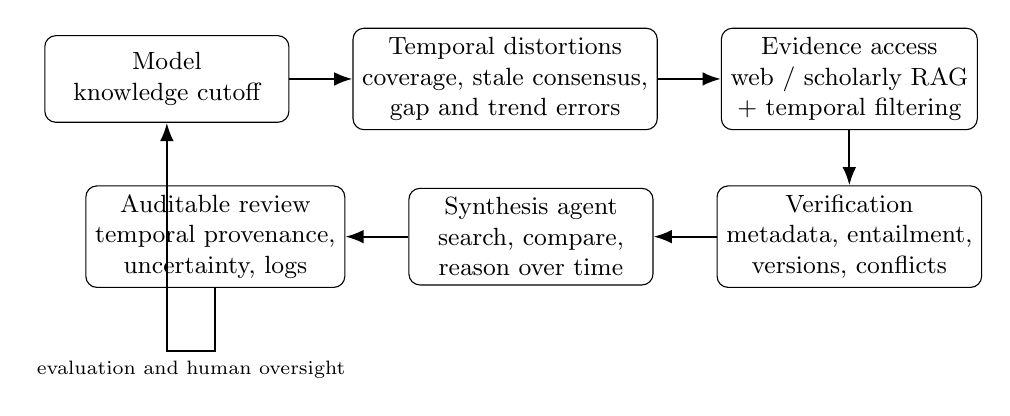
\begin{tikzpicture}[
  node distance=7mm and 8mm,
  box/.style={draw, rounded corners, align=center, minimum width=31mm, minimum height=11mm, font=\small},
  arrow/.style={-Latex, thick}
]
\node[box] (cutoff) {Model\\knowledge cutoff};
\node[box, right=of cutoff] (risk) {Temporal distortions\\coverage, stale consensus,\\gap and trend errors};
\node[box, right=of risk] (retrieve) {Evidence access\\web / scholarly RAG\\+ temporal filtering};
\node[box, below=of retrieve] (verify) {Verification\\metadata, entailment,\\versions, conflicts};
\node[box, left=of verify] (agent) {Synthesis agent\\search, compare,\\reason over time};
\node[box, left=of agent] (review) {Auditable review\\temporal provenance,\\uncertainty, logs};
\draw[arrow] (cutoff) -- (risk);
\draw[arrow] (risk) -- (retrieve);
\draw[arrow] (retrieve) -- (verify);
\draw[arrow] (verify) -- (agent);
\draw[arrow] (agent) -- (review);
\draw[arrow] (review.south) -- ++(0,-8mm) -| node[pos=.25,below,font=\scriptsize]{evaluation and human oversight} (cutoff.south);
\end{tikzpicture}
\caption{Taxonomy and workflow for temporally reliable LLM-generated literature reviews. The pipeline separates the source of temporal risk from retrieval, verification, synthesis, and audit stages.}
\Description{A six-stage horizontal workflow: model knowledge cutoff, temporal distortions, evidence access through scholarly retrieval and temporal filtering, verification, synthesis agent, and auditable review, with evaluation and human oversight feeding back to the cutoff stage.}
\label{fig:taxonomy}
\end{figure}

Figure~\ref{fig:taxonomy} summarizes the central architectural argument of this review: retrieval alone is
not sufficient. Temporal filtering, source-version tracking, claim verification, conflict handling, and human
oversight form complementary layers.

\begin{table*}[t]
\caption{Comparison of approaches for reducing knowledge-cutoff effects in literature-review systems.}
\label{tab:approaches}
\centering
\small
\begin{tabularx}{\textwidth}{p{0.15\textwidth}Y Y Y Y}
\toprule
\textbf{Approach} & \textbf{Freshness mechanism} & \textbf{Primary strength} & \textbf{Residual temporal risk} & \textbf{Reproducibility consideration} \\
\midrule
RAG \cite{lewis2020} & External corpus retrieval & Updates evidence without retraining & Stale or conflicting corpus entries & Store retrieved document IDs and timestamps \\
Scholarly RAG \cite{lala2023,asai2026} & Scientific full text and metadata & Better evidence grounding and citation support & Version ambiguity and retrieval bias & Preserve corpus version and ranking \\
Temporal filtering & Publication-date constraints & Explicit reference-time control & Publication date alone does not establish evidence quality & Record cutoff and filtering rule \\
Continual learning \cite{wu2024,shi2024} & Periodic parameter updates & New knowledge becomes internal & Forgetting and continuously changing model behavior & Version every model checkpoint \\
Knowledge editing \cite{yin2024} & Targeted representation updates & Efficient updates with historical knowledge preservation & Editing may interact with related facts & Record edit operations and model state \\
Agentic research \cite{du2025} & Iterative search and synthesis & Multi-step evidence gathering & Query drift, source bias, premature stopping & Log all searches, rankings, and prompts \\
Citation verification \cite{walters2023,davis2026} & Claim--reference checking & Detects bibliographic and support errors & Does not guarantee missing literature is found & Preserve verification outputs and evidence \\
\bottomrule
\end{tabularx}
\end{table*}

Table~\ref{tab:approaches} shows that the approaches address different failure modes. No single method
simultaneously guarantees freshness, temporal attribution, evidence completeness, and reproducibility.

\section{Research Challenges and Limitations}\label{sec:challenges}

\subsection{No universal definition of ``current''}\label{subsec:current}
A review can be current relative to its publication date, the last database search, a specified historical cutoff,
the latest peer-reviewed literature, the latest preprints, a field-specific guideline, or a dynamically changing
evidence base. Temporal correctness therefore requires an explicit reference time.

\subsection{Preprints and publication versions}\label{subsec:versions}
Rapidly evolving fields often rely heavily on preprints. A paper may exist as a preprint, a conference paper,
and later a journal version. A temporally accurate system should represent these as related versions rather
than independent pieces of evidence.

\subsection{Retractions and corrections}\label{subsec:retractions}
Scientific knowledge is not monotonically additive. New papers can invalidate earlier results through corrections,
retractions, failed replications, or improved methodologies. A ``latest paper wins'' strategy is therefore
inadequate. Temporal reasoning must be combined with evidence quality and scientific authority.

\subsection{Retrieval bias}\label{subsec:retrieval-bias}
RAG systems inherit biases from their retrieval corpus. If a corpus underrepresents journals, languages,
geographic regions, disciplines, or publication types, the generated review inherits those gaps. Retrieval can
therefore improve freshness without improving representativeness.

\subsection{Conflicting evidence}\label{subsec:conflicting-evidence}
Scientific fields rarely progress through simple replacement. Competing studies may coexist for years. An
LLM-generated review may collapse disagreement into a single narrative because generation rewards coherence.
This creates a tension between readability and epistemic fidelity.

\subsection{Citation correctness versus citation completeness}\label{subsec:citation-metrics}
A review can contain valid citations and still be poor if it omits major recent studies. Evaluation should therefore
distinguish citation correctness from evidence coverage. This distinction follows from the broader observation
that factuality and faithfulness do not fully capture the quality of scholarly synthesis \cite{maynez2020}.

\subsection{Evaluation benchmarks remain incomplete}\label{subsec:benchmarks}
EvolveBench and HoH are important steps toward temporal evaluation, but most benchmark designs still focus
on questions or individual answers rather than full literature-review generation \cite{zhu2025,ouyang2025}.
A review requires broader evaluation dimensions: search completeness, chronological coverage, citation
accuracy, claim-evidence alignment, synthesis quality, disagreement representation, methodological comparison,
gap identification, and reproducibility.

\subsection{Reproducibility}\label{subsec:reproducibility}
Dynamic retrieval creates a paradox: a system can become more current while becoming less reproducible. If
the same query is executed six months apart, the retrieved literature may differ. Scholarly use therefore
requires preservation of query strings, search date, database version, retrieved document IDs, document
versions, ranking results, model version, prompts, and generation settings.

\begin{figure}[t]
\centering
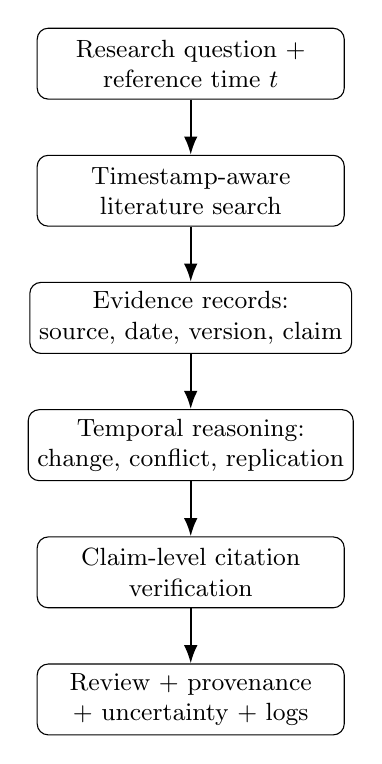
\begin{tikzpicture}[
  node distance=7mm,
  item/.style={draw, rounded corners, align=center, minimum width=39mm, minimum height=9mm, font=\small},
  arrow/.style={-Latex, thick}
]
\node[item] (q) {Research question +\\reference time $t$};
\node[item, below=of q] (search) {Timestamp-aware\\literature search};
\node[item, below=of search] (evidence) {Evidence records:\\source, date, version, claim};
\node[item, below=of evidence] (reason) {Temporal reasoning:\\change, conflict, replication};
\node[item, below=of reason] (cite) {Claim-level citation\\verification};
\node[item, below=of cite] (output) {Review + provenance\\+ uncertainty + logs};
\draw[arrow] (q) -- (search);
\draw[arrow] (search) -- (evidence);
\draw[arrow] (evidence) -- (reason);
\draw[arrow] (reason) -- (cite);
\draw[arrow] (cite) -- (output);
\end{tikzpicture}
\caption{Proposed temporal evidence lifecycle for a literature-review system. The reference time is established before retrieval and remains explicit through evidence selection, temporal reasoning, citation verification, and final reporting.}
\Description{A vertical workflow from research question and reference time, to timestamp-aware literature search, evidence records, temporal reasoning, claim-level citation verification, and a final review with provenance, uncertainty, and logs.}
\label{fig:evidence-lifecycle}
\end{figure}

Figure~\ref{fig:evidence-lifecycle} makes the reproducibility requirement explicit: the system should retain
an auditable chain from the research question and reference time to the evidence and final claims.

\section{Research Gaps and Future Directions}\label{sec:future}

\subsection{Temporal completeness as a formal evaluation metric}\label{subsec:temporal-completeness}
Current evaluation commonly emphasizes factual correctness and citation accuracy. Future literature-review
benchmarks should also measure temporal completeness. One possible metric is
\begin{equation}
    TC = \frac{\sum_{i=1}^{n} w_i I_i}{\sum_{i=1}^{n} w_i},
    \label{eq:temporal-completeness}
\end{equation}
where $w_i$ represents the importance of an expected publication or finding and $I_i\in\{0,1\}$ indicates
whether the review represents that item with appropriate temporal context. Equation~\eqref{eq:temporal-completeness}
distinguishes a review that is factually correct but incomplete from one that provides broad current coverage.
The metric is a proposed design concept rather than an established benchmark.

\subsection{Claim-level temporal provenance}\label{subsec:provenance}
Every substantive claim should ideally have a provenance tuple
\begin{equation}
    P=(\text{source},\text{date},\text{version},\text{evidence},\text{confidence}).
    \label{eq:provenance}
\end{equation}
This would enable a system to state not simply that a method is effective, but to describe the time window,
conditions, evidence strength, and remaining uncertainty. Equation~\eqref{eq:provenance} also provides a
natural unit for auditing generated reviews.

\subsection{Temporal knowledge graphs}\label{subsec:knowledge-graphs}
Future systems could represent literature as a temporal graph
\begin{equation}
    G_T=(V,E,T),
    \label{eq:temporal-graph}
\end{equation}
where nodes $V$ represent papers, methods, datasets, claims, and findings; edges $E$ represent citations,
comparisons, replications, contradictions, and extensions; and $T$ records temporal validity. Such a graph
would allow an LLM to reason over changes in relationships rather than merely retrieve documents.

\subsection{Temporal conflict resolution}\label{subsec:resolution}
Systems need explicit mechanisms for deciding what to do when sources disagree. A useful evidence hierarchy
can consider publication date, peer-review status, methodological quality, replication evidence,
retraction/correction status, sample size, domain authority, and directness of evidence. The latest source
should not automatically dominate.

\subsection{Time-aware research agents}\label{subsec:time-agents}
Future research agents should maintain a temporal state during search. Rather than simply accumulating sources,
the agent should ask when a claim was established, whether it subsequently changed, whether newer contradictory
evidence exists, whether a paper was available by the requested cutoff, whether it is a preprint or final
publication, and whether the result has been replicated. This would transform agents from document collectors
into temporal evidence synthesizers.

\subsection{Benchmarking literature reviews rather than individual answers}\label{subsec:review-benchmarks}
The field needs benchmark suites specifically designed for AI-generated literature reviews. Such benchmarks
should contain rapidly changing topics with known publication timelines and expert-created reference reviews.
Evaluation should measure the dimensions summarized in Table~\ref{tab:benchmark-dimensions}.

\begin{table}[t]
\caption{Proposed evaluation dimensions for temporally reliable literature reviews.}
\label{tab:benchmark-dimensions}
\centering
\small
\begin{tabularx}{\linewidth}{p{0.31\linewidth}Y}
\toprule
\textbf{Dimension} & \textbf{Core question} \\
\midrule
Temporal coverage & Did the system find important recent work? \\
Citation validity & Do cited papers exist and have correct metadata? \\
Citation entailment & Does each citation support the attached claim? \\
Temporal attribution & Is evidence placed in the correct historical context? \\
Trend fidelity & Does the review accurately describe field evolution? \\
Conflict representation & Are competing findings represented? \\
Gap validity & Are claimed gaps actually unresolved? \\
Reproducibility & Can another researcher reconstruct the review? \\
\bottomrule
\end{tabularx}
\end{table}

\subsection{Human-AI collaboration}\label{subsec:human-ai}
The evidence supports treating LLMs as research assistants rather than autonomous replacements for scholarly
judgment. The scoping review by Lieberum et al. found growing use across systematic-review tasks but limited
validation of unrestricted applications \cite{lieberum2025}. Human researchers remain important for assessing
methodological quality, interpreting contradictory findings, judging novelty, identifying disciplinary context,
evaluating source credibility, and determining whether a research gap is genuinely meaningful.

\subsection{Explicit uncertainty and abstention}\label{subsec:uncertainty}
An LLM should be able to report that the available evidence is insufficient to establish a consensus rather than
generating a confident synthesis from incomplete evidence. Gao et al. show that prompted knowledge cutoffs can
simulate temporal restrictions but do not fully prevent leakage from related post-cutoff information
\cite{gao2025}. Temporal awareness therefore cannot depend exclusively on prompting; systems need mechanisms
for verifying temporal admissibility.

\section{Conclusion}\label{sec:conclusion}
Knowledge cutoffs create a fundamental reliability problem for LLM-generated literature reviews in rapidly
evolving scientific fields. The problem is not limited to missing recent papers. A static knowledge boundary can
influence the perceived state of the field, distort citation patterns, preserve obsolete consensus, generate
false research gaps, and misrepresent emerging methodological trends.

The central insight is that scholarly synthesis is inherently temporal. A literature review describes not only
what is known, but when it became known, how evidence changed, which findings were superseded, and where
uncertainty remains. Conventional LLMs are optimized primarily for language prediction and general reasoning,
not for maintaining an auditable temporal model of scientific knowledge.

RAG provides an important architectural response by separating language-generation capabilities from external
knowledge storage. Scholarly systems such as PaperQA, LitLLM, automated review-generation pipelines, and
OpenScholar demonstrate increasingly sophisticated ways of combining retrieval with LLM-based synthesis
\cite{lala2023,agarwal2024,wu2025,asai2026}. Nevertheless, retrieval introduces its own temporal problems:
outdated documents can coexist with current ones, citation networks can privilege older literature, and
retrieval systems can fail to distinguish versions or conflicting findings.

Temporal benchmarks reinforce this conclusion. Research on evolving knowledge and outdated retrieval evidence
shows that temporal awareness remains an unresolved dimension even for capable systems
\cite{kim2024,zhu2025,ouyang2025}. Future literature-review systems should therefore treat time as a
first-class property of evidence. Reliable systems should combine timestamp-aware scholarly retrieval,
temporal provenance, claim-level citation verification, source-version tracking, conflict resolution,
uncertainty estimation, and reproducible search logs.

The goal should not be an LLM that merely produces a review that sounds current. It should be a research
system that can demonstrate why its review is current, which evidence supports each claim, when that evidence
was available, what evidence contradicts it, and what remains unknown. The architecture in Figure~\ref{fig:taxonomy}
and the evaluation dimensions in Table~\ref{tab:benchmark-dimensions} provide a compact representation of
this direction.

\section*{Acknowledgments}
The author acknowledges the use of the previously submitted manuscript as the basis for this revised review
paper and the ACM/Overleaf template as the formatting reference specified for the course activity.

\bibliographystyle{ACM-Reference-Format}
\bibliography{references}

\end{document}
